%--------------------------------------------------------------------------
% @file informe_final.tex
%
% @date 09/04/16 22:51:05
% @author Martin Noblia
% @email martin.noblia@openmailbox.org
%
% @brief
% Informe final de Sistemas digitales
% @detail
%
% Licence:
% This program is free software: you can redistribute it and/or modify
% it under the terms of the GNU General Public License as published by
% the Free Software Foundation, either version 3 of the License, or (at
% your option) any later version.
% 
% This program is distributed in the hope that it will be useful, but
% WITHOUT ANY WARRANTY; without even the implied warranty of
% MERCHANTABILITY or FITNESS FOR A PARTICULAR PURPOSE.  See the GNU
% General Public License for more details.
% 
% You should have received a copy of the GNU General Public License
%
%---------------------------------------------------------------------------
% Start
%---------------------------------------------------------------------------
\documentclass[10pt]{article}
%---------------------------------------------------------------------------
% Packages
%---------------------------------------------------------------------------
\usepackage{amsmath}
\usepackage{tikz}
\usepackage{epigraph}
\usepackage{lipsum}
\usepackage{hyperref} 
\usepackage{listings}
\usepackage{fancyhdr}
\usepackage[utf8]{inputenc}
\usepackage{hyperref} 
\usepackage[spanish]{babel}
\usepackage{amsmath}
\usepackage{amsthm}
\usepackage{amssymb}
\usepackage{latexsym}
\usepackage{graphicx}
\usepackage{color}
\usepackage{moredefs}
\usepackage{fancybox}
\usepackage{subfig}
\usepackage{float}
\usepackage{xcolor}
\usepackage{wallpaper}
\usepackage{textcomp}
\usepackage{minted} % for syntax highlight
\usepackage{textcomp} % for the TradeMark shit
%---------------------------------------------------------------------------
% Definitions
%---------------------------------------------------------------------------
\oddsidemargin -0.2in \textwidth 7.0in \topmargin -0.9in \textheight
9.0in
\parindent 3em
%---------------------------------------------------------------------------
% Cut of Spanish words
%---------------------------------------------------------------------------
\hyphenation{e-jem-plo
e-rro-res de-pen-dien-te co-rrien-te res-pues-ta fi-gu-ran
cons-tan-tes o-pe-ra-cion i-lu-mi-na-cion}
%---------------------------------------------------------------------------
% Page styles
%---------------------------------------------------------------------------
\pagestyle{fancy}
\headheight 50pt 
\renewcommand{\arrayrulewidth}{3pt} 
\newtheorem{defi}{{\it Definición}}[section]
%---------------------------------------------------------------------------
% Header page
%---------------------------------------------------------------------------
\rhead{\includegraphics[width=.075\textwidth]{./Images/logo_iaci2.eps}} % iaci logo
\chead{}
\lhead{Sistemas Digitales}
\rfoot{1º cuatrimestre 2016  }
\cfoot{\thepage}
\lfoot{\bf{Universidad Nacional de Quilmes}}
%---------------------------------------------------------------------------
% Colors
%---------------------------------------------------------------------------
\definecolor{azul-claro}{rgb}{0.335,0.89,1}
\definecolor{gainsboro}{rgb}{0.86,0.86,0.86}
\definecolor{mediumseagreen}{rgb}{0.24,0.7,0.44}
\definecolor{moccasin}{rgb}{1,0.89,0.71}
\definecolor{cornflowerblue}{rgb}{0.39,0.58,0.93}
\definecolor{lightgray}{rgb}{0.83,0.83,0.83}
\definecolor{darkgrey}{rgb}{0.66,0.66,0.66}
\definecolor{darkslategray}{rgb}{0.18,0.31,0.31}
\definecolor{lavender}{rgb}{0.9,0.9,0.98}
\definecolor{azure}{rgb}{0.94,1,1}
\definecolor{honeydew}{rgb}{0.94,1,0.94}
%---------------------------------------------------------------------------
% Custom section header(this shit generate a box color)
%---------------------------------------------------------------------------
\renewcommand{\arrayrulewidth}{1pt} 
\newcommand{\mcaja}[1]{%
{{\fboxsep 10pt \fboxrule 1pt%
\fcolorbox{black}{lightgray}{%
\color{black} \Huge #1}}}
}
\newcommand{\nuevobox}[1]{%
{{\fboxsep 14pt \fboxrule 1pt%
\fcolorbox{black}{darkgrey}{%
\color{lavender} \huge #1}}}
}
\newcommand{\ssection}[1]{\section[#1]{\mcaja{#1}}}
\makeatletter
\newcommand{\sect}[1]{\subsection[#1]{\nuevobox{#1}}}
\makeatletter
\def\section{\@ifstar\unnumberedsection\numberedsection}
\def\numberedsection{\@ifnextchar[%]
\numberedsectionwithtwoarguments\numberedsectionwithoneargument}
\def\unnumberedsection{\@ifnextchar[%]
\unnumberedsectionwithtwoarguments\unnumberedsectionwithoneargument}
\def\numberedsectionwithoneargument#1{\numberedsectionwithtwoarguments[#1]{#1}}
\def\unnumberedsectionwithoneargument#1{\unnumberedsectionwithtwoarguments[#1]{#1}}
\def\numberedsectionwithtwoarguments[#1]#2{%
\ifhmode\par\fi
\removelastskip
\vskip 3ex\goodbreak
\refstepcounter{section}%
\begingroup
%\noindent
\leavevmode\large\bfseries\raggedright\mcaja%%
\thesection\ #2\par\nobreak
\endgroup
\noindent\hrulefill\nobreak
\vskip 2ex\nobreak
\addcontentsline{toc}{section}{%
\protect\numberline{\thesection}%
#1}%
}
\def\unnumberedsectionwithtwoarguments[#1]#2{%
\ifhmode\par\fi
\removelastskip
\vskip 3ex\goodbreak
% \refstepcounter{section}%
\begingroup
\noindent
\leavevmode\Large\bfseries\raggedright
% \thesection\
#2\par\nobreak
\endgroup
\noindent\hrulefill\nobreak
\vskip 0ex\nobreak
\addcontentsline{toc}{section}{%
%
\protect\numberline{\thesection}%
#1}%
}
\makeatother
%%%Cap\’itulos
\usepackage{helvet}
%\usepackage{psboxit,pstcol}
\makeatletter
\def\@makechapterhead#1{%
{\parindent \z@ \raggedright \reset@font
\hbox to \hsize{%
\rlap{\raisebox{-2.5em}{\raisebox{\depth}{%%% Necesita la imagen "imgCapitulo"
\includegraphics[width=10em]{./Images/logo_iaci2.eps}}}}%
\rlap{\hbox to 6em{\hss
\reset@font\sffamily\fontsize{8em}{8em}\selectfont\black
\thechapter\hss}}%
\hspace{10em}%
\vbox{%
\advance\hsize by -10em
\reset@font\fontfamily{hv}\bfseries\Large
#1
\par
}%
}}%
\vskip 5pt
\hrulefill
\vskip 50pt
}
%---------------------------------------------------------------------------
% Redefinition of Theorems and Corollarys
%---------------------------------------------------------------------------
\makeatother
\newtheorem{theorem}{Teorema}[section]
\newtheorem{corollary}{Corolario}[theorem]
\newtheorem{lemma}[theorem]{Lema}
%---------------------------------------------------------------------------
% Title Page decoration
%---------------------------------------------------------------------------
\definecolor{titlepagecolor}{cmyk}{.3,.73,0,.37}


\newcommand\titlepagedecoration{%
\begin{tikzpicture}[remember picture,overlay,shorten >= -10pt]

\coordinate (aux1) at ([yshift=-15pt]current page.north east);
\coordinate (aux2) at ([yshift=-410pt]current page.north east);
\coordinate (aux3) at ([xshift=-4.5cm]current page.north east);
\coordinate (aux4) at ([yshift=-150pt]current page.north east);

\begin{scope}[titlepagecolor!40,line width=12pt,rounded corners=12pt]
\draw
  (aux1) -- coordinate (a)
  ++(225:5) --
  ++(-45:5.1) coordinate (b);
\draw[shorten <= -10pt]
  (aux3) --
  (a) --
  (aux1);
\draw[opacity=0.6,titlepagecolor,shorten <= -10pt]
  (b) --
  ++(225:2.2) --
  ++(-45:2.2);
\end{scope}
\draw[titlepagecolor,line width=8pt,rounded corners=8pt,shorten <= -10pt]
  (aux4) --
  ++(225:0.8) --
  ++(-45:0.8);
\begin{scope}[titlepagecolor!70,line width=6pt,rounded corners=8pt]
\draw[shorten <= -10pt]
  (aux2) --
  ++(225:3) coordinate[pos=0.45] (c) --
  ++(-45:3.1);
\draw
  (aux2) --
  (c) --
  ++(135:2.5) --
  ++(45:2.5) --
  ++(-45:2.5) coordinate[pos=0.3] (d);   
\draw 
  (d) -- +(45:1);
\end{scope}
\end{tikzpicture}%
}


\newcommand*{\plogo}{\fbox{$\mathcal{PL}$}}
\newcommand*{\titleGP}{\begingroup % Create the command for including the title page in the document
\centering % Center all text
\vspace*{\baselineskip} % White space at the top of the page

\rule{\textwidth}{1.6pt}\vspace*{-\baselineskip}\vspace*{2pt} % Thick horizontal line
\rule{\textwidth}{0.4pt}\\[\baselineskip] % Thin horizontal line

{\LARGE Sistemas Digitales\\[0.3\baselineskip] Trabajo Final:\\[0.3\baselineskip] \textit{ Desarrollo de Firmware para estacion meteorologica}}\\[0.2\baselineskip] % Title

\rule{\textwidth}{0.4pt}\vspace*{-\baselineskip}\vspace{3.2pt} % Thin horizontal line
\rule{\textwidth}{1.6pt}\\[\baselineskip] % Thick horizontal line

\scshape % Small caps
 Martín Noblía
\vspace*{2\baselineskip} % Whitespace between location/year and editors

Profesores: \\[\baselineskip]
{\Large Jose Juarez\\ Eric Pernia\par}
\vfill % Whitespace between editor names and publisher logo_iaci2
\includegraphics[width=.175\textwidth]{./Images/logo_iaci2.eps}

% Editor list
{\itshape Universidad Nacional de Quilmes \par} % Editor affiliation

\vfill % Whitespace between editor names and publisher logo

%\plogo \\[0.3\baselineskip] % Publisher logo
{\scshape 2016} \\[0.3\baselineskip] % Year published
%{\large THE PUBLISHER}\par % Publisher

\endgroup}
%---------------------------------------------------------------------------
% Begin of the document
%---------------------------------------------------------------------------
\begin{document}
\pagestyle{empty} 

\titleGP
\titlepagedecoration


\newpage
\pagestyle{fancy}

\section{Introduccion}
Las estaciones Meteorologicas son una serie de sensores que actuan en conjunto para estimar
variables referidas al clima, como ser:
\begin{itemize}
   \item Temperaturas
   \item Direccion del viento
   \item velocidad del viento
   \item Humedad
   \item Si esta lloviendo (sensor de lluvia)
\end{itemize}
Estas variables son muy importantes para los procesos productivos donde su productividad depende de las condiciones climaticas.
\begin{itemize}
   \item Viniedos
   \item Granjas
   \item Campos de agricultura
\end{itemize}

\begin{figure}[H]
   \centering
   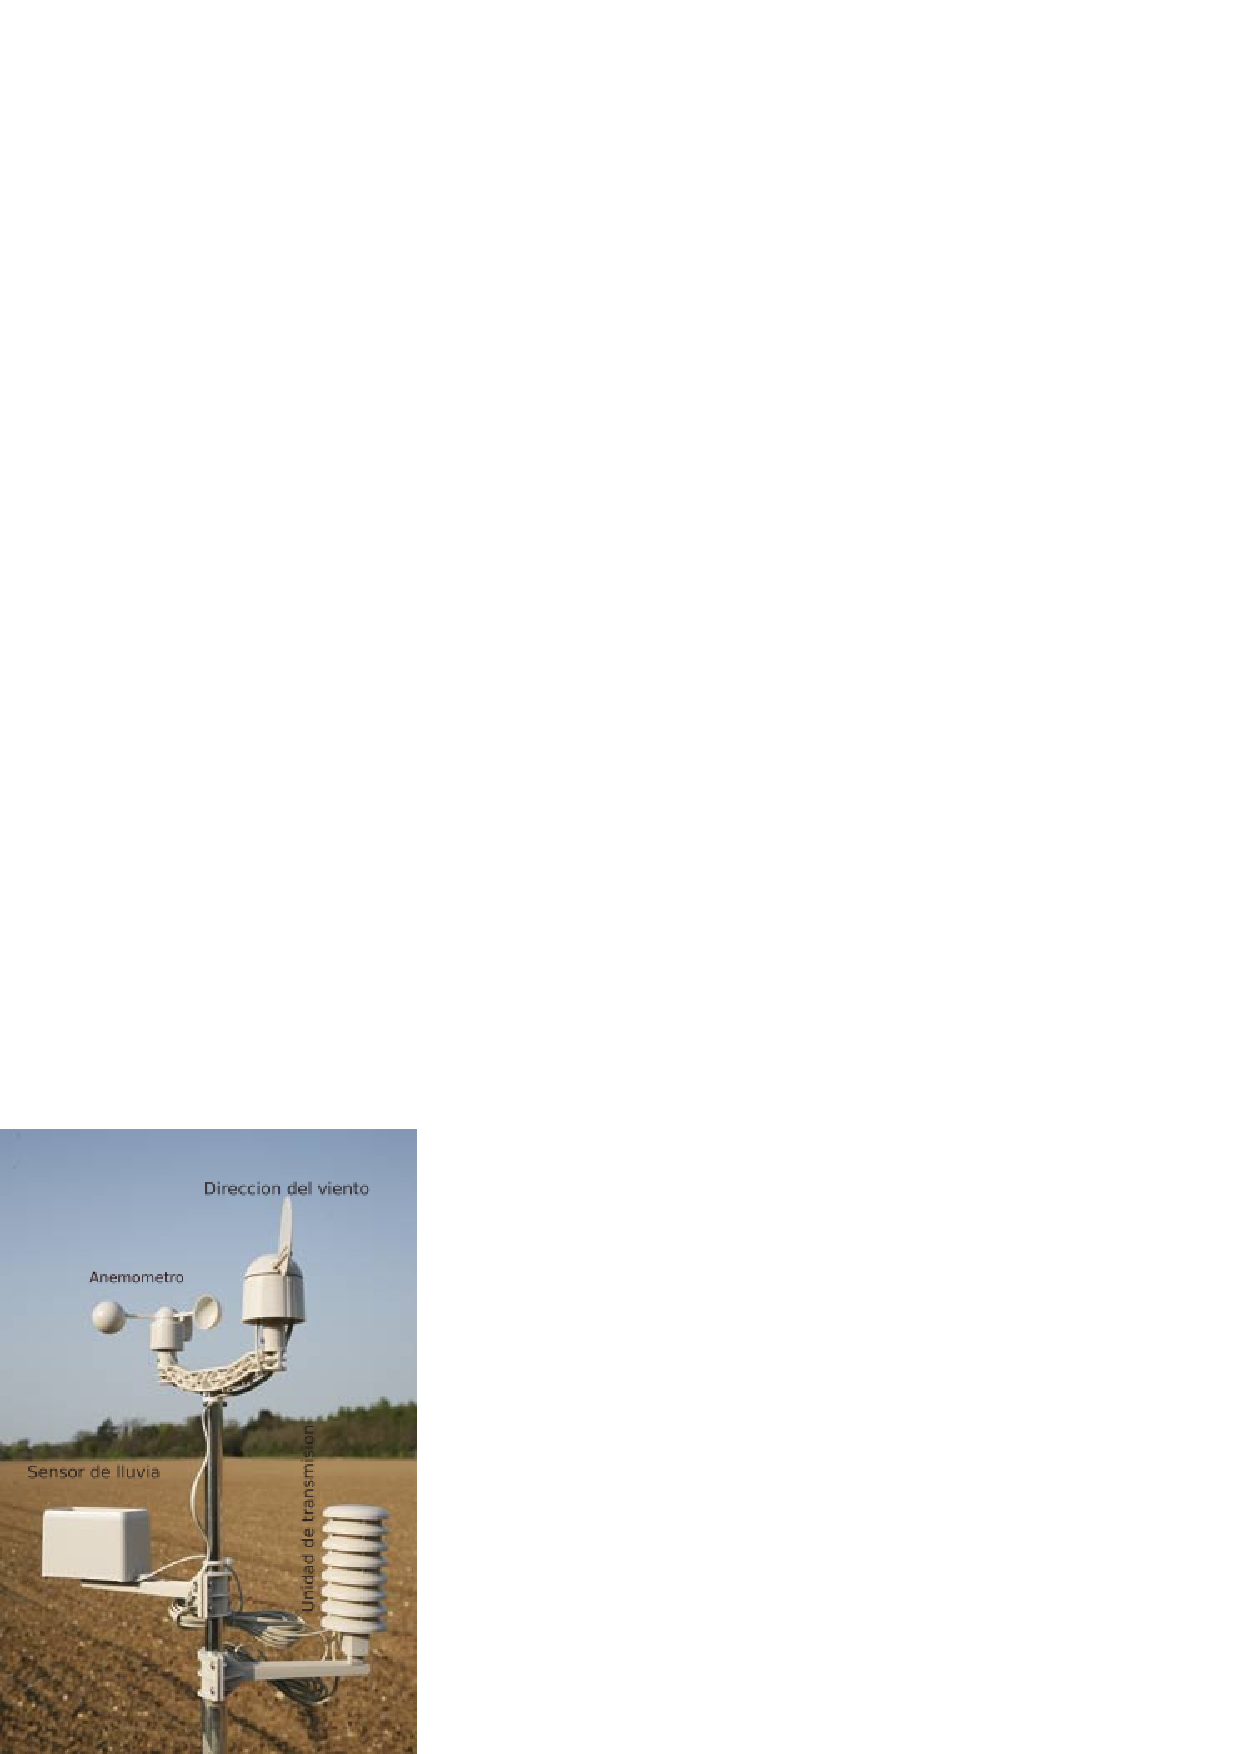
\includegraphics[width=0.37\textwidth]{./Images/station_farm.png}
   \caption{Estacion meteorologica en Campo}\label{fig:station_farm}
\end{figure}
En este trabajo nos centraremos en el desarrollo del firmware\footnote{\url{ https://es.wikipedia.org/wiki/Firmware }}de dos de ellos: Un sensor de velocidad del viento y un sensor de direccion de viento. Este ultimo ademas posee una intefaz visibles con leds.


\section{Descripcion del sistema}

En el siguiente diagrama podemos ver como se relaciona cada componente del sistema:
\begin{figure}[H]
   \centering
   \includegraphics[width=0.37\textwidth]{./Images/rect4136.png}
   \caption{Diagrama esquematico del sistema}\label{fig:diagrama_esquematico}
\end{figure}

\begin{itemize}
   \item Sensor de direccion del viento: Consta de una veleta que gira al soplar el viento, en su interior posse 8 sensores magneticos\footnote{\url{https://en.wikipedia.org/wiki/Reed_switch}}, un iman que gira solidario a la veleta y un circuito (divisor resistivo) que entrega una salida analogica.
               \begin{figure}[H]
                  \centering
                  \includegraphics[width=0.27\textwidth]{./Images/winddir1.jpg}
                  \caption{Sensor de direccion del viento por dentro (circuito interno)}\label{fig:veleta_por_dentro}
               \end{figure}
               \begin{figure}[H]
                  \centering
                  \includegraphics[width=0.27\textwidth]{./Images/winddir2.jpg}
                  \caption{Sensor de direccion del viento por dentro despiezado}\label{fig:veleta_por_dentro2}
               \end{figure}
   \item Sensor de velocidad del viento: Consta de un simple sensor magneticos y un iman como el de el anterior sensor que entrega valores de alto o bajo que pueden ser leidos como entrada digital en la placa.
               \begin{figure}[H]
                  \centering
                  \includegraphics[width=0.27\textwidth]{./Images/windspeed1.jpg}
                  \caption{Sensor de velocidad del viento por dentro}\label{fig:anemometro}
               \end{figure}
               \begin{figure}[H]
                  \centering
                  \includegraphics[width=0.37\textwidth]{./Images/windspeed2.jpg}
                  \caption{Sensor de velocidad del viento despiezado}\label{fig:anemometro2}
               \end{figure}
   \item Leds de direccion del viento: Con esta interfaz podemos visualizar en que estado esta el sensor de direccion del viento
               \begin{figure}[H]
                  \centering
                  \includegraphics[width=0.37\textwidth]{./Images/leds.png}
                  \caption{Interfaz grafica del sensor de direccion del viento a base de leds}\label{fig:leds}
               \end{figure}
   \item Buzzer: Se encarga de emitir una alarma cuando un evento ha ocurrido (ver la seccion 3 para mas detalles).
   \item Interfaz Grafica de Usuario: Se encarga de mostrar los valores de velocidad y direccion del viento que le fueron entregados por puerto serie (UART)
   \item Edu-CIAA\footnote{\url{http://proyecto-ciaa.com.ar/}}: Es una placa de desarrollo de Hardware y software abierto, la cual cuenta con las siguientes caracteristicas tecnicas:
               \begin{figure}[H]
                  \centering
                  \includegraphics[width=0.37\textwidth]{./Images/edu_ciaa.jpg}
                  \caption{Caracteristicas tecnicas de la Edu-CIAA}\label{fig:edu_ciaa}
               \end{figure}
               \begin{figure}[H]
                  \centering
                  \includegraphics[width=0.37\textwidth]{./Images/edu-ciaa-nxp.png}
                  \caption{Edu-CIAA-NXP}\label{fig:edu_ciaa-nxp}
               \end{figure}

\end{itemize}



\section{Disenio del Firmware}
Las especificaciones que debe realizar nuestro sistema son:

\begin{itemize}
   \item Calcular la velocidad del viento mediante la lectura del sensor correspondiente
   \item Calcular la direccion del viento mediante la lectura del sensor correspondiente
   \item Encender los leds correspondientes de acuerdo a la direccion calculada
   \item Activar una alarma en caso de que la velocidad del viento sea mas elevada que un umbral elegido
   \item Mostrar los resultados mediante una GUI(\textit{Graphical User Interface}) en una PC conectada a la placa
\end{itemize}

Para el desarrollo del firmware se utlizaron dos Componentes principales:
\begin{itemize}
   \item FreeRTOS\texttrademark\footnote{\url{http://www.freertos.org/}}: Es el Sistema operativo de tiempo real mas utilizado en el mundo de los sistemas embebidos 
      \begin{itemize}
         \item En FreeRTOS\texttrademark cada hilo de ejecucion se llama task(tarea)
         \item El FreeRTOS\texttrademark para LPC17xx incluye todas las funcionalidades del standard
         \item Podemos operar en modo \textit{pre-emptive} y en modo *co-operative*
         \item Asignacion de prioridad de tareas flexible
         \item Colas(\textit{Queues})
         \item Semaforos binarios
         \item Semaforos contadores
         \item Semaforos recursivos
         \item \textit{mutexes}
         \item Funciones \textit{Tick hook}
         \item Funciones \textit{Idle hook}
         \item Chequeo de \textit{Stackoverflow}
         \item macros \textit{Trace hook}
      \end{itemize}
   \item Libreria de abtraccion \textit{HAL} sAPI\footnote{\url{https://github.com/epernia/sAPI}} Nos permite interactuar con la placa de desarrollo a un nivel de abstraccion mas alto, esto hace que el desarrollo de prototipos como es este proyecto sea mas rapido
\end{itemize}

Ya que utilizamos FreeRTOS\texttrademark nuestro disenio se basa en programar las tareas(\textit{tasks}),  como interactuan entre ellas. Para poder visualizar mejor estas relaciones tenemos el siguiente grafico:
\begin{figure}[H]
   \centering
   \includegraphics[width=0.57\textwidth]{./Images/Tasks.png}
   \caption{Diagrama de relacion de tareas}\label{fig:Task}
\end{figure}
Pasamos a detallar cada una de las tareas:

\begin{itemize}
   \item \verb|prvTimeControllerTask|: Esta tarea se encarga de llevar una cuenta precisa del tiempo(ya que utiliza un delay exacto provisto por FreeRTOS\texttrademark \verb|vTaskDelayUntil|\footnote{\url{http://www.freertos.org/vtaskdelayuntil.html}}) una vez que ha llegado el tiempo(1 segundo) envia una
      senial a la tarea que esta calculando la frecuencia con que ha girado el sensor de velocidad del viento. Codigo:
      \begin{minted}{c}
         void prvTimeControllerTask(void *pvParameters)
         {
            portTickType xLastWakeTime;
            xLastWakeTime = xTaskGetTickCount();
            while(1)
            {
               vTaskDelayUntil( &xLastWakeTime, (SIGNAL_MESSAGE_PERIOD / portTICK_RATE_MS));
               xSemaphoreGive(xTimeSignal);

            }

         }
      \end{minted}
   \item\verb|prvAnemometerTask|: Esta tarea es la encargada de calcular la frecuencia de giro del sensor del viento. Cada segundo le llega un mensage de tiempo ahi es cuando envia lo calculado a la tarea que se encarga de administrar el periferico UART, antes de volver a empezar \textit{resetea} los valores calcualdos, ademas verifica si el valor calculado en mayor que un umbral, en caso de serlo envia una senial a una tarea de alarma. Codigo:
      \begin{minted}{c}
         
         void prvAnemometerTaks(void *pvParameters)
         {
            /* Anemometer pin states */
            typedef enum{PIN_UP, PIN_FALLING, PIN_DOWN, PIN_RISING} pin_state_t;
            /* Auxiliar variables */
            portBASE_TYPE xFreq = 0;
            portBASE_TYPE xCounter = 0;
            portBASE_TYPE xTemp = 0;
            /* initial condition */
            pin_state_t pin_state = PIN_UP;
            /* message data */
            xMetaData xAnemometerMessage;
            /* message flag for the Gatekeeper */
            xAnemometerMessage.xSource = SENDER_ANEMOMETER;
            /* Task processig */
            while(1)
            {

               /* MEF for counting the states changes */
               switch(pin_state)
               {
                  case PIN_UP:
                     {
                        if(!digitalRead(DIO32))
                        {
                           pin_state = PIN_FALLING;
                        }
                        break;
                     }
                  case PIN_FALLING:
                     {
                        xCounter += 3;
                        if(!digitalRead(DIO32))
                        {
                           pin_state = PIN_DOWN;
                           xFreq++;
                           digitalWrite(LEDR, ON);
                        }
                        else
                           pin_state = PIN_UP;
                        break;
                     }
                  case PIN_DOWN:
                        {
                        if(digitalRead(DIO32))
                        {
                           pin_state = PIN_RISING;
                        }
                        break;
                     }
                  case PIN_RISING:
                     {
                        xCounter += 3;
                        if(digitalRead(DIO32))
                        {
                           pin_state = PIN_UP;
                           digitalWrite(LEDR, OFF);
                        }
                        else
                        {
                           pin_state = PIN_DOWN;
                        }
                        break;
                      }
                  }

               if(xSemaphoreTake(xTimeSignal, ( TickType_t )0))
               {
                  if(xFreq > FREQUENCY_ALARM_THRESHOLD_1)
                  {
                     xTemp = ALARM_MESSAGE_1;
                     xQueueSendToBack(xALARMQueue, (void *)&xTemp, portMAX_DELAY);
                  }
                  if(xFreq > FREQUENCY_ALARM_THRESHOLD_2)
                  {
                     xTemp = ALARM_MESSAGE_2;
                     xQueueSendToBack(xALARMQueue, (void *)&xTemp, portMAX_DELAY);
                  }
                  /* The time message arrive --> prepare the message package */
                  xAnemometerMessage.xMessage = xFreq;
                  /* send the package via the Gatekeeper */
                  xQueueSendToBack(xUARTQueue, (void *)&xAnemometerMessage, ( TickType_t )0);
                  /* reset the values */
                  xFreq = 0;
                  xCounter = 0;
               }
            }

         }
      \end{minted}
   \item \verb|vUartGateKeeperTask|: Esta tarea se encarga de administrar el periferico UART mediante una cola que solo tiene el poder de enviar datos al periferico por ella, ademas por como fueron diseniados los datos que maneja, estos pueden provenir de distintas fuentes. Asi \textit{Gatekeeper} puede disernir de donde provienen los datos y actuar en consecuencia. Ademas envia los datos a la PC de tal manera que sean facilmente \textit{parseables} por la aplicacion que los recibe. Codigo:
      \begin{minted}{c}

         void vUartGatekeeperTask( void *pvParameters )
         {
            xMetaData xReceived;
            portBASE_TYPE xStatus;

               while(1)
               {
                  /* Wait for a message to arrive. */
                  xStatus = xQueueReceive(xUARTQueue, &xReceived, portMAX_DELAY);

                  if(xStatus == pdPASS)
                  {
                     switch(xReceived.xSource)
                     {
                        case SENDER_ANEMOMETER:
                           {
                              vPrintStringAndNumber("Freq:", xReceived.xMessage);
                              break;
                           }
                        case SENDER_WIND_ROSE:
                           {
                              vPrintStringAndNumber("State:", xReceived.xMessage);
                              break;
                           }
                        /* case SENDER_PC: */
                        /*    { */
                        /*       break; */
                        /*    } */
                     }
                  }
                  else
                  {
                     vPrintString("Error!!!");
                  }

               }
         }
      \end{minted}
   \item \verb|prvWindRoseGetDirection|: Esta tarea se encarga de leer los datos analogicos del sensor de direccion de viento y asigna de acuerdo a una tabla dada por el fabricante el estado en que se encuentra el sensor. Ademas una vez que ha detectado el estado en cual se encuentra envia ese dato a una funcion auxiliar que mapea estados con pines, de acuerdo al fabricante de el visor de leds. Codigo:
      \begin{minted}{c}
         void prvWindRoseGetDirection(void *pvParameters)
         {
            /* initial state */
            wind_states_t wind_states = N;
            /* task metadata message for the Gatekeeper */
            xMetaData xWindRoseMessage;
            xWindRoseMessage.xSource = SENDER_WIND_ROSE;
            portBASE_TYPE uartBuff[10];
            portBASE_TYPE sample = 0;

            while(1)
            {
               vTaskDelay(WIND_ROSE_POOLING_PERIOD / portTICK_RATE_MS);
               /* read the analog sensor value */
               sample = analogRead(AI0);
               /* convert the sample to decimal number */
               itoa(sample, uartBuff, 10);
               /* N */
               if(CHECK(sample, N_MIN, N_MAX))
               {
                  wind_states = N;
                  do_state(wind_states);
               }
               /* NNO */
               if(CHECK(sample, NNO_MIN, NNO_MAX))
               {
                  wind_states = NNO;
                  do_state(wind_states);
               }
               /* NO */
               if(CHECK(sample, NO_MIN, NO_MAX))
               {
                  wind_states = NO;
                  do_state(wind_states);
               }
               /* NOO */
               if(CHECK(sample, NOO_MIN, NOO_MAX))
               {
                  wind_states = NOO;
                  do_state(wind_states);
               }
               /* O */
               if(CHECK(sample, O_MIN, O_MAX))
               {
                  wind_states = O;
                  do_state(wind_states);
               }
               /* SOO */
               if(CHECK(sample, SOO_MIN, SOO_MAX))
               {
                  wind_states = SOO;
                  do_state(wind_states);
               }
               /* SO */
               if(CHECK(sample, SO_MIN, SO_MAX))
               {
                  wind_states = SO;
                  do_state(wind_states);
               }
               /* SSO */
               if(CHECK(sample, SSO_MIN, SSO_MAX))
               {
                  wind_states = SSO;
                  do_state(wind_states);
               }
               /* S */
               if(CHECK(sample, S_MIN, S_MAX))
               {
                  wind_states = S;
                  do_state(wind_states);
               }
               /* SSE */
               if(CHECK(sample, SSE_MIN, SSE_MAX))
               {
                  wind_states = SSE;
                  do_state(wind_states);
               }
               /* SE */
               if(CHECK(sample, SE_MIN, SE_MAX))
               {
                  wind_states = SE;
                  do_state(wind_states);
               }
               /* SEE */
               if(CHECK(sample, SEE_MIN, SEE_MAX))
               {
                  wind_states = SEE;
                  do_state(wind_states);
               }
               /* E */
               if(CHECK(sample, E_MIN, E_MAX))
               {
                  wind_states = E;
                  do_state(wind_states);
               }
               /* NEE */
               if(CHECK(sample, NEE_MIN, NEE_MAX))
               {
                  wind_states = NEE;
                  do_state(wind_states);
               }
               /* NE */
               if(CHECK(sample, NE_MIN, NE_MAX))
               {
                  wind_states = NE;
                  do_state(wind_states);
               }
               /* NNE */
               if(CHECK(sample, NNE_MIN, NNE_MAX))
               {
                  wind_states = NNE;
                  do_state(wind_states);
               }

               xWindRoseMessage.xMessage = wind_states;
               xQueueSendToBack(xUARTQueue, (void *)&xWindRoseMessage, ( TickType_t )0);

            }
         }
      \end{minted}
   \item \verb|prvAlarmActivateTask|: Esta tarea es una alarma que espera a que sea puesto en la cola un mensage de alarma(por la tarea \verb|prvAnemometerTask|) por el momento pueden \textit{setearse} dos niveles de umbral(y por consiguiente dos mensages que entiende cuando son recibidos). Al recibir alguno de los mensages activa un \textit{buzzer} con distintas alarmas para cada uno. Codigo:
      \begin{minted}{c}
         
            prvAlarmActivateTask(void *pvParameters)
            {
               portBASE_TYPE xTemp;

               while(1)
               {
                  vTaskDelay(ALARM_POOLING_PERIOD / portTICK_RATE_MS);
                  xQueueReceive(xALARMQueue, &xTemp,  portMAX_DELAY);
                  if(xTemp == ALARM_MESSAGE_1)
                  {
                     digitalWrite(DIO11, ON);
                     vTaskDelay(ALARM_BEEP_WARNIG_PERIOD / portTICK_RATE_MS);
                     digitalWrite(DIO11, OFF);
                  }
                  if(xTemp == ALARM_MESSAGE_2)
                  {
                     digitalWrite(DIO11, ON);
                     vTaskDelay(ALARM_BEEP_DESASTER / portTICK_RATE_MS);
                     digitalWrite(DIO11, OFF);
                     digitalWrite(DIO11, ON);
                     vTaskDelay(ALARM_BEEP_DESASTER / portTICK_RATE_MS);
                     digitalWrite(DIO11, OFF);
                  }
               }


            }
      \end{minted}
   \item GUI: Se programo una aplicacion en Python con la libreria Kivy\footnote{\url{https://kivy.org/}}, la cual recibe los datos de la UART y de acuerdo a que estado y frecuencia que recibio realiza:
      \begin{itemize}
         \item Calcula la velocidad del viento en $Km/h$. Ya que recibe la frecuencia por segundo en que esta girando el sensor de velocidad puede hacer una simple multiplicacion y convertir los datos, la constante de conversion es: $\frac{1 tick}{seg} \approx 2.4 \frac{Km}{h}$
         \item Actualiza la pantalla con los datos del estado en que se encuentra el sensor de direccion del viento.
      \end{itemize}
\end{itemize}

\section{Resultados}

Se logro el objetivo principal que era tener un firmware que adquiriera la informacion de los sensores en tiempo real. El sistema es flexible en al agregado de nuevos sensores ya que se ha modularizado el codigo de tal manera que sea facil la inclusion de nuevos componentes.


\section{Trabajos a futuro}
Como trabajos a futuro o cosas para mejorar de la implementacion:
\begin{itemize}
   \item Implementar la cuenta de \textit{Ticks} con una interrupcion, la cual solo tendria que actualizar un contador (\verb|xFrec++|) y cuando le sea enviada la senial de tiempo activar un mensage a la tarea de \textit{Gatekeeper}
   \item Permitir al usuario a traves de la GUI ingresar el/los valores umbrales de alarma.
   \item Hacer que la conexion entre los sensores y la placa sea remota
   \item Hacer un \textit{dataloger} con los datos obtenidos.
\end{itemize}
\newpage



%------------------------------------------------------------------------- 
% Bibliografia 
%-------------------------------------------------------------------------
\begin{thebibliography}{6} \bibitem{Principal}{Using The FreeRTOS\texttrademark Real Time Kernel. Richard Barry}\\ \bibitem{Principal2}{Real Time Systems and Design. Phillip Laplante}
\end{thebibliography} 

\end{document}
